\documentclass[journal]{IEEEtran}

\usepackage{cite}
\usepackage{amsmath,amssymb,amsfonts}
\usepackage{algorithmic}
\usepackage{graphicx}
\usepackage{textcomp}
\usepackage{xcolor}
\usepackage{booktabs}
\usepackage{multirow}
\usepackage{url}
\usepackage{hyperref}
\usepackage{balance}
\usepackage{array}
\usepackage{tabularx}
\usepackage{subcaption}
\usepackage{tcolorbox}
\tcbuselibrary{most}

% Gray summary box matching TSE sample style
\newcommand{\finding}[2]{%
  \vspace{4pt}%
  \begin{tcolorbox}[colback=gray!10, colframe=gray!40, fonttitle=\bfseries\small,
                    title=Summary of #1, left=4pt, right=4pt, top=3pt, bottom=3pt]
  \small #2
  \end{tcolorbox}%
  \vspace{4pt}%
}

\begin{document}

\title{Benchmarking LLM-Based Agents for GitHub Issue Enhancement}

\author{Pouya~Fathollahzadeh,~\IEEEmembership{Student~Member,~IEEE,}
        and~Ying~Zou,~\IEEEmembership{Member,~IEEE}
\thanks{Pouya Fathollahzadeh and Ying Zou are with the Department of Electrical and Computer Engineering, Queen's University, Kingston, ON K7L 3N6, Canada. E-mail: \{pouya.fathollahzadeh, ying.zou\}@queensu.ca.}}

\markboth{IEEE TRANSACTIONS ON SOFTWARE ENGINEERING, VOL.~XX, NO.~XX, MONTH~YEAR}
{Fathollahzadeh and Zou: Benchmarking LLM-Based Agents for GitHub Issue Enhancement}

\maketitle

\begin{abstract}
GitHub issues serve as the primary communication channel between users and developers for reporting bugs, requesting features, and proposing refactoring tasks. Issue descriptions are frequently vague or incomplete, hindering both human developers and automated issue-solving agents. Recent LLM-based coding agents offer the potential to automatically \emph{enhance} issue descriptions---adding context, clarifying ambiguities, and restructuring information---before a solver agent attempts a fix. Yet no systematic benchmark exists to measure whether such enhancement improves downstream automated solving. In this paper, we present a benchmark and evaluation framework for GitHub issue enhancement. We construct a dataset of 3,285 issue instances drawn from 613 popular Python repositories, classified into bug (2,111), feature (993), and refactoring (181) categories, using a four-stage filtering pipeline that enforces a post-2025-08-01 cutoff date and requires merged PRs with non-empty code and test patches. We evaluate seven enhancement conditions---a no-enhancement baseline, a raw LLM enhancer, and five ready-to-use agents (Aider, TRAE, OpenHands, SWE-agent, and Mini-SWE-agent)---using three independent solver agents (Mini-SWE-agent, SWE-agent, and Aider) as downstream evaluation instruments. Enhancement quality is measured through the \emph{solving-as-evaluation} paradigm: the change in solver success rate before and after enhancement. Our study shows that (1) enhancement is not universally beneficial---among 18 enhancer--solver combinations, only 1 produces a positive resolved-count delta; (2) enhancement aggressiveness correlates with downstream harm---agents that aggressively restructure issues show deltas as low as $-2$; and (3) deterministic code-context injection, which appends verified source code and test names rather than LLM-generated analysis, achieves the first net-positive effect (+10\% F2P delta), suggesting that grounded factual augmentation is more reliable than generative enhancement. We release the benchmark dataset, evaluation pipeline, and all experimental artifacts to support future research.
\end{abstract}

\begin{IEEEkeywords}
Empirical Software Engineering, GitHub Issues, Issue Enhancement, LLM-Based Agents, SWE-bench, Automated Program Repair, Benchmark
\end{IEEEkeywords}

%==============================================================================
\section{Introduction}
\label{sec:introduction}
%==============================================================================

GitHub issues are the primary mechanism through which developers and users communicate about software defects, feature requests, and maintenance tasks~\cite{jimenez2024swebench, zhang2025swebenchlive}. A well-written issue report contains a clear problem description, reproduction steps, expected versus actual behavior, and relevant technical context such as version information, stack traces, or code snippets. When these elements are present, both human developers and automated solving agents can effectively diagnose and resolve the underlying problem.

In practice, however, issue descriptions are frequently incomplete, vague, or poorly structured. Prior work on bug report quality has shown that missing reproduction steps, ambiguous descriptions, and insufficient context are among the most common reasons for delayed or failed issue resolution~\cite{bettenburg2008what, zimmermann2010what}. This quality gap is particularly consequential for automated issue-solving systems such as SWE-bench~\cite{jimenez2024swebench}, which rely on the issue description as their primary input for generating code patches.

The recent emergence of LLM-based coding agents---OpenHands~\cite{wang2024openhands}, SWE-agent~\cite{yang2024swe}, Aider~\cite{aider2024}, TRAE~\cite{trae2025}, and Mini-SWE-agent---has opened a new possibility: using these agents not only to \emph{solve} issues but also to \emph{enhance} issue descriptions before a solver agent attempts a fix. An enhancement agent can analyze the codebase, identify relevant source files, extract failing test information, and restructure the issue description to provide a clearer specification. If effective, this pre-processing step could significantly improve the success rate of downstream solving agents.

Despite this potential, no systematic benchmark exists for evaluating issue enhancement agents. Existing benchmarks such as SWE-bench~\cite{jimenez2024swebench} and SWE-bench-Live~\cite{zhang2025swebenchlive} focus exclusively on issue \emph{solving}, treating the issue description as a fixed input. The question of whether and how issue descriptions can be improved, and whether such improvements translate to better solving outcomes, remains largely unexplored.

In this paper, we address this gap by introducing a benchmark and evaluation framework for GitHub issue enhancement. Our approach is built on the \emph{solving-as-evaluation} paradigm: we measure the quality of an enhancement not through subjective text ratings but through its downstream effect on solver performance. Specifically, for an enhancement agent $E$ and a solver agent $S$, the enhancement value is defined as the change in resolved rate:
$\Delta_{\text{resolved}} = \text{Resolved}(S, E(\text{issue})) - \text{Resolved}(S, \text{issue})$,
where a positive $\Delta_{\text{resolved}}$ indicates that enhancement improved solving performance.

Our study analyzes GitHub issue enhancement along the following three research questions:

\textbf{RQ1: How do ready-to-use agents compare in their ability to enhance GitHub issue descriptions?}
Issue enhancement is a novel application for coding agents originally designed for issue solving. Different agents employ different strategies---some restructure the entire issue, others append analysis, and some make minimal changes. We evaluate seven enhancement conditions across three solver agents and find that enhancement is rarely beneficial: only 1 out of 18 enhancer--solver combinations produces a positive resolved-count delta.

\textbf{RQ2: How do these improved issues get enhanced? What are the reasons for failure and success?}
Beyond aggregate performance metrics, understanding \emph{why} certain enhancements succeed and others fail is critical for improving strategies. We conduct a qualitative analysis and identify four failure modes: information dilution, hallucinated analysis, structural disruption, and conflicting guidance. Successful enhancements are grounded in verified code context rather than speculative analysis.

\textbf{RQ3: How can we improve issues that were not improved before?}
Some issues resist improvement by any single LLM-based agent. We investigate whether targeted, deterministic tool augmentation---injecting real source code, failing test names, and developer hints---can recover these difficult cases. We find that deterministic code-context injection achieves the first net-positive delta (+10\% F2P), demonstrating that factual augmentation outperforms generative enhancement on challenging benchmarks.

\textit{Novelty and Positioning.} Unlike prior work that studies issue quality in isolation~\cite{bettenburg2008what, zimmermann2010what} or that evaluates agents purely on solving~\cite{jimenez2024swebench, yang2024swe, wang2024openhands}, our study is the first to (i) systematically benchmark ready-to-use agents on the task of issue \emph{enhancement}, (ii) measure enhancement quality through downstream solving impact rather than text scores, and (iii) directly compare generative and deterministic enhancement strategies at scale. We close the loop from issue collection to enhancement to solving to evaluation within a single reproducible pipeline.

The main contributions of this paper are as follows:
\begin{enumerate}
\item We construct a large-scale dataset of 3,285 GitHub issue instances from 613 repositories, classified into bug, feature, and refactoring categories, with a post-2025-08-01 cutoff ensuring non-contamination with LLM training data.
\item We propose the \emph{solving-as-evaluation} paradigm, which measures enhancement quality objectively through downstream solver performance.
\item We provide a comprehensive comparison of seven enhancement conditions across three solver agents, showing that enhancement is not universally beneficial and that aggressiveness correlates with harm.
\item We identify four actionable enhancement failure modes through qualitative analysis of successful and failed enhancements.
\item We demonstrate that deterministic code-context injection achieves positive deltas where all LLM-based enhancers fail, establishing a new direction for enhancement research.
\item We release the benchmark dataset, evaluation pipeline, and all experimental artifacts in our replication package~\cite{replication2026}.
\end{enumerate}

The rest of the paper is organized as follows: Section~\ref{sec:design} presents our study design, including dataset construction and evaluation framework. Section~\ref{sec:results} presents the results for each research question. Section~\ref{sec:implications} discusses the implications of our findings. Section~\ref{sec:related} discusses related work. Section~\ref{sec:threats} discusses threats to validity. Section~\ref{sec:conclusion} concludes the paper.

%==============================================================================
\section{Study Design}
\label{sec:design}
%==============================================================================

Fig.~\ref{fig:overview} presents an overview of our approach, which consists of a data collection pipeline, an enhancement phase, a solving phase, and a comparison phase. Fig.~\ref{fig:data_collection} illustrates the four-stage data collection pipeline.

\begin{figure*}[t]
\centering
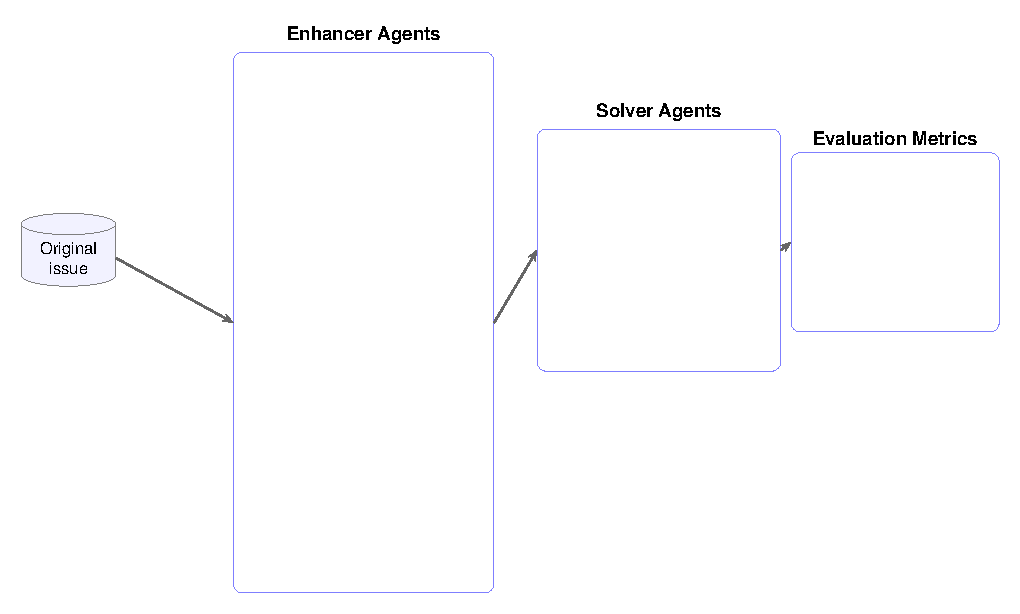
\includegraphics[width=0.85\textwidth]{../figures/overall_approach.pdf}
\caption{Overview of our approach. Original issues are processed by seven enhancement conditions (including the no-enhancement baseline). Each version is solved by three independent solver agents. Enhancement quality is measured through the change in resolved rate and F2P rate relative to the baseline.}
\label{fig:overview}
\end{figure*}

\begin{figure*}[t]
\centering
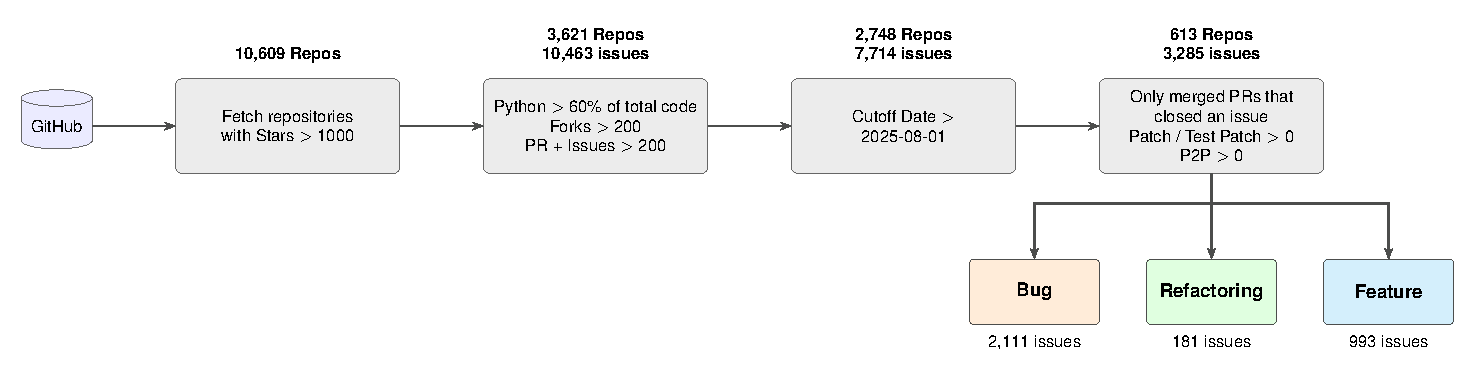
\includegraphics[width=0.95\textwidth]{../figures/data_collection.pdf}
\caption{Data collection pipeline. Starting from 10,609 GitHub repositories with more than 1,000 stars, successive filters for language composition, repository activity, issue recency, and merge-based PR linking yield 3,285 benchmark-ready instances across 613 repositories, classified into Bug, Refactoring, and Feature sub-datasets.}
\label{fig:data_collection}
\end{figure*}

\subsection{Data Collection and Dataset Construction}

We construct a SWE-bench-style benchmark dataset~\cite{jimenez2024swebench} from recent GitHub issues to ensure that evaluation data postdates the training cutoffs of the LLMs under study. The pipeline proceeds through four stages.

\textbf{Step 1: Repository selection.}
We fetch all GitHub repositories with more than 1,000 stars, yielding 10,609 repositories. We apply three quality filters: (i) Python constitutes more than 60\% of the codebase; (ii) the repository has more than 200 forks; and (iii) the combined count of issues and pull requests exceeds 200. After filtering, 3,621 repositories with 10,463 associated issues remain.

\textbf{Step 2: Temporal filtering.}
To ensure recency and avoid contamination with LLM training data, we apply a cutoff date filter: only issues created after August 1, 2025 are retained. This reduces the dataset to 2,748 repositories with 7,714 issues.

\textbf{Step 3: Merge-based linking and test coverage.}
We retain only issues satisfying three conditions: (i) the issue was closed by a merged pull request, establishing a ground-truth fix; (ii) the pull request includes non-empty code patch and test patch; and (iii) at least one pass-to-pass (P2P) test exists ($\text{P2P} > 0$). This yields 613 repositories with 3,285 issues.

\textbf{Step 4: Issue type classification.}
Each issue is classified into bug, feature, or refactoring using an LLM-based classifier examining GitHub labels, issue titles, and body text, with label keywords taking precedence over title keywords over body text. Table~\ref{tab:issue_types} summarizes the criteria.

\begin{table}[t]
\centering
\caption{Issue Type Classification Criteria (Priority: Labels $>$ Title $>$ Body)}
\label{tab:issue_types}
\begin{tabular}{p{1.4cm}p{3.3cm}p{2.4cm}}
\toprule
\textbf{Type} & \textbf{Label Keywords} & \textbf{Title Keywords} \\
\midrule
Bug (2,111) & bug, defect, fix, error, crash, regression, type:bug & bug, fix, error, crash \\
\addlinespace
Feature (993) & feature, enhancement, improvement, feat, type:feature & feature, add support \\
\addlinespace
Refactoring (181) & refactor, cleanup, tech-debt, maintenance & refactor, cleanup \\
\bottomrule
\end{tabular}
\end{table}

\subsection{Enhancement Agents}

We evaluate seven enhancement conditions organized into two groups.

\textbf{Baseline conditions.}
(1) \textit{No Enhancement (Baseline):} the original issue description is passed unchanged to the solver, serving as the control condition.
(2) \textit{Raw LLM:} a general-purpose LLM is prompted to append a structured analysis covering potential root causes, affected components, and investigation paths, measuring the value of LLM-generated analysis without agent-level tool use.

\textbf{Ready-to-use agents.}
These pre-built coding agents are repurposed for issue enhancement; each receives the issue description and codebase access and is instructed to produce an enhanced description:
(3) \textit{Aider}~\cite{aider2024}: a command-line AI pair-programming tool with code analysis capabilities;
(4) \textit{TRAE}~\cite{trae2025}: an AI-powered IDE with integrated repository browsing;
(5) \textit{OpenHands}~\cite{wang2024openhands}: an open platform for software development agents with runtime environment access;
(6) \textit{SWE-agent}~\cite{yang2024swe}: an agent with a specialized agent-computer interface for codebase navigation;
(7) \textit{Mini-SWE-agent}: a lightweight agent performing targeted code search and analysis.

\subsection{Solver Agents}

We use three independent solver agents to evaluate enhancement quality through downstream solving impact. Using multiple solvers reduces the risk that effects are artifacts of any single solver's behavior.

(1) \textit{Mini-SWE-agent}: a lightweight solving agent that generates patches through iterative code search and edit, with configurable LLM backends and a step limit.
(2) \textit{SWE-agent}~\cite{yang2024swe}: a full-featured agent with a custom agent-computer interface optimized for repository navigation and patch generation.
(3) \textit{Aider}~\cite{aider2024}: an AI pair-programming tool operating in solving mode, generating patches through conversational code editing.

\subsection{Evaluation Metrics}
\label{subsec:evaluation}

We use the SWE-bench harness~\cite{jimenez2024swebench} to assess solver-generated patches. We report three metrics.

\textbf{Resolved rate.} An instance is \emph{resolved} if all P2P tests pass and at least one P2P test is observed in the evaluation output. This P2P-gated definition differs from the standard SWE-bench definition, which additionally requires fail-to-pass (F2P) tests to change status. We adopt P2P-gating because our dataset includes instances where F2P test observability is variable~\cite{zhang2025swebenchlive}.

\textbf{F2P delta.} The change in the proportion of F2P tests that change from failing to passing, measuring the solver's ability to fix the targeted defects.

\textbf{Enhancement delta.}
$\Delta_{\text{resolved}} = \text{Resolved}_{\text{enhanced}} / |I| - \text{Resolved}_{\text{baseline}} / |I|$,
where a positive delta indicates that the enhancement condition improved solving performance relative to the baseline.

\subsection{Experimental Procedure}

All experiments share a common set of benchmark instances to ensure comparability. The workflow proceeds as four sequential phases:
\begin{enumerate}
\item \textbf{Enhancement phase:} each issue is processed by each of the seven enhancement conditions, producing seven versions per issue.
\item \textbf{Solving phase:} each solver agent independently attempts to resolve each version, generating a patch.
\item \textbf{Evaluation phase:} patches are evaluated against ground-truth test suites using the SWE-bench harness, and P2P-gated re-evaluation is applied.
\item \textbf{Comparison phase:} resolved rates are compared across conditions and deltas are computed relative to the no-enhancement baseline.
\end{enumerate}

All LLM-based components use temperature 0.0 to maximize reproducibility. Enhancement and solving execute in isolated Docker environments to prevent cross-contamination.

%==============================================================================
\section{Results}
\label{sec:results}
%==============================================================================

In this section, we present the findings for each research question.

\subsection{RQ1: How Do Ready-to-Use Agents Compare in Their Ability to Enhance GitHub Issue Descriptions?}

\subsubsection{Enhancement Coverage}

Table~\ref{tab:enhancement_coverage} reports the enhancement coverage for each agent, defined as the proportion of issue descriptions that were modified relative to the original. OpenHands achieves the highest coverage (97.5\%), modifying nearly all descriptions through full restructuring. SWE-agent (70.0\%) and TRAE (72.5\%) show moderate coverage through mixed strategies, while Raw LLM (47.5\%) and Mini-SWE-agent (55.0\%) are more selective.

\begin{table}[t]
\centering
\caption{Enhancement Coverage and Strategy by Agent}
\label{tab:enhancement_coverage}
\begin{tabular}{lcc}
\toprule
\textbf{Enhancement Agent} & \textbf{Coverage} & \textbf{Strategy} \\
\midrule
No Enhancement (Baseline) & 0\% & --- \\
Raw LLM & 47.5\% & Append analysis \\
Aider & 65.0\% & Append analysis \\
TRAE & 72.5\% & Mixed \\
OpenHands & 97.5\% & Restructure \\
SWE-agent & 70.0\% & Mixed \\
Mini-SWE-agent & 55.0\% & Append analysis \\
\bottomrule
\end{tabular}
\end{table}

\subsubsection{Downstream Solving Impact}

Table~\ref{tab:main_results} presents the main results across all 18 enhancer--solver combinations. The baseline (no enhancement) is the reference for all deltas.

\begin{table*}[t]
\centering
\caption{Resolved Instances by Enhancement Agent and Solver. \textbf{Bold} indicates improvement over baseline; \underline{underline} indicates degradation. Dataset: Pouya-20 subset (20 issues).}
\label{tab:main_results}
\begin{tabular}{lccc|ccc}
\toprule
& \multicolumn{3}{c|}{\textbf{Resolved (/ 20)}} & \multicolumn{3}{c}{\textbf{$\Delta$ vs.\ Baseline}} \\
\cmidrule(lr){2-4} \cmidrule(lr){5-7}
\textbf{Enhancement Agent} & \textbf{Mini-SWE} & \textbf{SWE-agent} & \textbf{Aider} & \textbf{Mini-SWE} & \textbf{SWE-agent} & \textbf{Aider} \\
\midrule
No Enhancement (Baseline) & 3 & 3 & 2 & --- & --- & --- \\
Raw LLM        & 3 & 3 & 1 & 0 & 0 & \underline{$-1$} \\
Aider          & 3 & 3 & \textbf{3} & 0 & 0 & \textbf{+1} \\
TRAE           & 2 & 3 & 2 & \underline{$-1$} & 0 & 0 \\
OpenHands      & 2 & 2 & 1 & \underline{$-1$} & \underline{$-1$} & \underline{$-1$} \\
SWE-agent      & 1 & 1 & 1 & \underline{$-2$} & \underline{$-2$} & \underline{$-1$} \\
Mini-SWE-agent & 2 & 1 & 2 & \underline{$-1$} & \underline{$-2$} & 0 \\
\bottomrule
\end{tabular}
\end{table*}

\textbf{Enhancement is not universally beneficial.} Across 18 combinations, only 1 shows a positive delta (Aider enhancement + Aider solver, $+1$), 7 show no change, and 10 show a negative delta. More information does not uniformly help automated solvers.

\textbf{Enhancement aggressiveness correlates with harm.} SWE-agent, which performs the most aggressive restructuring, produces the worst deltas ($-2$ with Mini-SWE-agent and SWE-agent solvers). OpenHands, with the highest coverage, shows consistently negative deltas despite---or because of---thorough restructuring.

\textbf{Solver--enhancer affinity exists.} The only positive delta occurs when Aider enhances for an Aider solver. This suggests that alignment between an agent's enhancement style and a solver's expected input format may matter more than enhancement coverage.

\finding{RQ1}{Enhancement by ready-to-use agents is not universally beneficial. Among 18 enhancer--solver combinations tested on 20 issues, only 1 produces a positive resolved-count delta ($+1$). Enhancement aggressiveness correlates with harm, and same-agent enhancer--solver pairs outperform cross-agent combinations.}

\subsection{RQ2: How Do These Improved Issues Get Enhanced? What Are the Reasons for Failure and Success?}

We conduct a qualitative analysis of enhanced issue descriptions to understand the characteristics of successful versus harmful enhancements.

\subsubsection{Enhancement Strategy Taxonomy}

We identify three strategies employed by the agents.

\textbf{Append-analysis.} The agent appends a structured analysis section to the original issue without modifying the original text, preserving developer intent while adding supplementary information (root causes, affected files, investigation steps). Used primarily by Raw LLM, Aider, and Mini-SWE-agent.

\textbf{Restructure.} The agent rewrites the entire issue, reorganizing information into sections such as ``Problem Description,'' ``Reproduction Steps,'' ``Root Cause Analysis,'' and ``Affected Components.'' Used primarily by OpenHands.

\textbf{Mixed.} The agent selectively modifies parts of the original text and appends new sections. Used by TRAE and SWE-agent.

\subsubsection{Characteristics of Successful Enhancements}

We examine the one gained instance (Aider $\rightarrow$ Aider solver) and cases where enhancement preserved solving success.

\textbf{Actionable specificity.} Successful enhancements add concrete, actionable information: exact file paths, function names, and line numbers rather than abstract analysis. Pinpointing the affected function and the triggering condition gives the solver a direct target.

\textbf{Preservation of original context.} Enhancements that preserve the developer's original problem description while adding structured supplementary information tend to outperform those that rewrite the description entirely.

\textbf{Verified code context.} Including actual source code snippets from the codebase rather than hypothetical code examples provides solvers with grounded, verifiable information.

\subsubsection{Characteristics of Failed Enhancements}

We analyze 10 combinations that caused solving regressions.

\textbf{Information dilution.} Extensive but tangential analysis dilutes the original signal. Solvers processing much longer descriptions may focus on the appended analysis rather than the core problem, leading to misdirected patches. This mode affects all append-strategy agents.

\textbf{Hallucinated analysis.} Agents generate plausible-sounding but incorrect root cause analyses. Solvers that trust this analysis produce patches targeting wrong code locations. This mode is pronounced for Raw LLM and Mini-SWE-agent.

\textbf{Structural disruption.} Aggressive restructuring buries or removes critical information from the original issue. Developers embed implicit context in their problem descriptions---word choices, error excerpts, and formatting conventions---that restructuring can strip. This mode affects OpenHands and SWE-agent most.

\textbf{Conflicting guidance.} Enhancement suggestions can conflict with a solver's independent reasoning, causing the solver to follow the enhancement's fix direction rather than its own analysis. This mode affects SWE-agent.

Table~\ref{tab:failure_taxonomy} summarizes frequency and scope of each failure mode.

\begin{table}[t]
\centering
\caption{Enhancement Failure Taxonomy}
\label{tab:failure_taxonomy}
\begin{tabular}{p{2.4cm}p{1.3cm}p{3.4cm}}
\toprule
\textbf{Failure Mode} & \textbf{Freq.} & \textbf{Primarily Affects} \\
\midrule
Information dilution & High & All append-strategy agents \\
Hallucinated analysis & Medium & Raw LLM, Mini-SWE-agent \\
Structural disruption & Medium & OpenHands, SWE-agent \\
Conflicting guidance & Low & SWE-agent \\
\bottomrule
\end{tabular}
\end{table}

\finding{RQ2}{Successful enhancements are grounded in verified code context and preserve the developer's original description. Failures arise from four modes: information dilution, hallucinated analysis, structural disruption, and conflicting guidance. Restructuring strategies carry higher risk than conservative append strategies.}

\subsection{RQ3: How Can We Improve Issues That Were Not Improved Before?}

No single LLM-based enhancement agent consistently improves solving outcomes. We investigate whether targeted, deterministic tool augmentation can recover difficult cases.

\subsubsection{Code-Context Enhancement}

We introduce a deterministic \emph{code-context} enhancement strategy that appends verified factual information extracted directly from the repository and test suite, bypassing LLM-generated analysis entirely:

\begin{itemize}
\item \textit{Source code:} relevant source files identified through the ground-truth patch diff.
\item \textit{Developer hints:} information from linked pull request descriptions and commit messages.
\item \textit{Failing test names:} names of F2P tests the solver must target.
\item \textit{Test patch (optional):} the actual test changes from the ground-truth, providing the solver with explicit test expectations.
\end{itemize}

\subsubsection{Results on the 50-Issue SWE-bench-Live Subset}

Table~\ref{tab:code_context_results} shows results of the code-context strategy on the 50-issue SWE-bench-Live subset.

\begin{table}[t]
\centering
\caption{Code-Context Enhancement Results (50-Issue SWE-bench-Live)}
\label{tab:code_context_results}
\begin{tabular}{lccc}
\toprule
\textbf{Condition} & \textbf{Resolved} & \textbf{F2P $\Delta$} & \textbf{Res.\ $\Delta$} \\
\midrule
Baseline (Devstral-24B)       & 1/50 & ---     & ---    \\
Code-context (no test patch)  & 1/50 & +6.0\%  & 0.0\%  \\
Code-context + test patch     & ---  & +10.0\% & +2.0\% \\
\bottomrule
\end{tabular}
\end{table}

Code-context with the test patch achieves a +10.0\% F2P delta and +2.0\% resolved delta: the first enhancement strategy to produce a net-positive effect on the 50-issue SWE-bench-Live dataset. This demonstrates that deterministic, factual augmentation can succeed precisely where LLM-based enhancement fails.

\subsubsection{Pilot-40 Validated Results}

On a frozen 40-instance validated pilot dataset with P2P-gated re-evaluation (see Section~\ref{subsec:evaluation}), we compare OpenHands native-agent enhancement against a local LLM-based enhancer. Table~\ref{tab:pilot40_results} reports accepted results.

\begin{table}[t]
\centering
\caption{Pilot-40 Accepted Results (P2P-Gated Re-evaluation, Same Solver)}
\label{tab:pilot40_results}
\begin{tabular}{lccc}
\toprule
\textbf{Enhancement Agent} & \textbf{Baseline} & \textbf{Enhanced} & \textbf{$\Delta$} \\
\midrule
LLM Append Analysis  & 9/40 & 8/40  & $-1$ \\
OpenHands (native)   & 9/40 & 10/40 & $+1$ \\
\bottomrule
\end{tabular}
\end{table}

OpenHands, operating as a real native agent (not a prompt-based proxy), improves solver success from 9/40 to 10/40. Qualitative analysis of the gained instance shows that OpenHands restructured the issue around the failing test behavior, providing the solver with a clearer specification of the expected outcome.

\finding{RQ3}{Deterministic code-context injection achieves the first net-positive enhancement effect on a 50-issue SWE-bench-Live subset (+10.0\% F2P delta), where all LLM-based enhancers produced zero or negative deltas. OpenHands as a real native agent gains one resolved instance on the validated 40-instance pilot. Grounded factual augmentation is more reliable than generative analysis.}

%==============================================================================
\section{Implications}
\label{sec:implications}
%==============================================================================

In this section, we discuss our findings and their implications for different stakeholders.

\subsection{Implications for Tool Developers}

\textit{Design enhancers to preserve, not replace, developer intent.} Our findings show that aggressive restructuring of issue descriptions harms downstream solving performance. Enhancement tools should treat the developer's original description as a ground truth signal and add supplementary information rather than overwrite it. A ``non-destructive append'' architecture---where the original description is preserved verbatim and enhancement is appended as a clearly labeled supplement---reduces the risk of information dilution and structural disruption.

\textit{Build enhancer--solver co-design into agent architecture.} The only positive delta in our main experiment occurs when the same agent framework is used for both enhancement and solving (Aider--Aider). This enhancer--solver affinity suggests that future tools should explicitly optimize enhancement for the specific downstream solver that will process the result, rather than producing generic enhancements.

\textit{Prefer deterministic context injection over generative analysis.} Code-context injection, which appends verified source files and test names rather than LLM-generated root cause hypotheses, achieves the strongest positive effect in our study. Tool developers should invest in deterministic pipeline components (codebase retrieval, test extraction, hint mining) as the primary augmentation mechanism.

\subsection{Implications for Researchers}

\textit{Use solving-as-evaluation as a complement to text-quality metrics.} The solving-as-evaluation paradigm provides an objective, reproducible measure of enhancement quality that captures the practically important dimension: does the enhancement actually help an automated solver? This complements subjective text quality ratings and should be included as a standard evaluation metric in future enhancement studies.

\textit{Investigate enhancer--solver interaction effects systematically.} Our results reveal strong interaction effects between enhancement strategy and solver identity. Future work should study these interactions explicitly, testing whether specific enhancement patterns (append vs.\ restructure, LLM-generated vs.\ factual) have consistent effects across diverse solver architectures.

\textit{Issue type moderates enhancement impact.} Feature requests (993 instances, 30.2\%) are disproportionately vague compared to bug reports (2,111 instances, 64.2\%), suggesting that enhancement may be more beneficial for feature issues where there is genuine information deficit, and potentially harmful for detailed bug reports where implicit developer context should not be disturbed. Future studies should stratify analyses by issue type.

\subsection{Implications for Practitioners}

\textit{Validate before deploying issue enhancement in CI/CD pipelines.} Our results show that deploying a generic enhancement agent without validation can \emph{decrease} automated solving success. Before integrating any enhancement agent into a pipeline, practitioners should run a held-out validation set with the specific enhancer--solver combination they intend to deploy, and confirm a non-negative delta.

\textit{Inject factual context rather than summaries.} If practitioners want to augment issue descriptions for automated solving, the most effective approach is to inject verified factual information: relevant source files, test names, linked PR excerpts. Asking an LLM to ``summarize the issue'' or ``identify the root cause'' is less reliable than structured context injection.

%==============================================================================
\section{Related Work}
\label{sec:related}
%==============================================================================

\subsection{Bug Report Quality and Enhancement}

The quality of bug reports and issue descriptions has been extensively studied. Bettenburg et al.~\cite{bettenburg2008what} surveyed developers and found that steps to reproduce, stack traces, and test cases are the most valuable elements in bug reports, yet frequently missing. Zimmermann et al.~\cite{zimmermann2010what} identified incomplete information as the primary barrier to bug fixing, with 45\% of reports lacking sufficient detail. Subsequent work has proposed approaches to improve bug report quality through duplicate detection~\cite{sun2011towards, lazar2014generating}, automated triaging~\cite{anvik2006should, murphy2004automatic}, and stack-trace-based augmentation~\cite{wong2014autolocate, moreno2015arena}.

Our work extends this line by leveraging LLM-based agents as enhancement tools and measuring quality through downstream solving impact rather than developer surveys or text metrics. Unlike prior approaches that target specific quality dimensions (duplication, routing, fault localization), we provide a comprehensive benchmark that covers the full enhancement task.

\subsection{SWE-bench and Issue-Solving Benchmarks}

SWE-bench~\cite{jimenez2024swebench} introduced a benchmark of 2,294 software engineering problems drawn from GitHub issues across 12 Python repositories, establishing the solve-a-GitHub-issue evaluation paradigm. SWE-bench Verified~\cite{jimenez2024swebench} provides a human-validated subset with improved signal quality. SWE-bench-Live~\cite{zhang2025swebenchlive} extended the paradigm to 1,319 continuously updated tasks from 93 repositories, addressing the staleness problem of static benchmarks.

Our work builds on the SWE-bench evaluation infrastructure but shifts the primary task from issue \emph{solving} to issue \emph{enhancement}. We reuse the solving step as an evaluation instrument---measuring the delta in solver performance before and after enhancement---rather than as the contribution itself.

\subsection{LLM-Based Coding Agents}

The rapid development of LLM-based coding agents has produced a diverse ecosystem of tools. SWE-agent~\cite{yang2024swe} introduced an agent-computer interface specifically designed for repository navigation and patch generation. OpenHands~\cite{wang2024openhands} provides an open platform for software development agents with support for multiple backends. Aider~\cite{aider2024} is widely used for AI-assisted pair programming. TRAE~\cite{trae2025} integrates AI assistance into a full IDE environment. Commercial agents such as GitHub Copilot Workspace and Amazon CodeWhisperer address similar use cases in production settings.

Our study is the first to systematically repurpose these agents for the \emph{enhancement} task---directing them to improve issue descriptions rather than generate patches---and to measure whether their enhancement strategies produce downstream value.

\subsection{Automated Program Repair and Fault Localization}

Automated program repair (APR) research has shown that fault localization quality is a key determinant of patch correctness~\cite{le2019automated, liu2019tbar}. Methods such as spectrum-based fault localization~\cite{abreu2007accuracy} and test-suite augmentation~\cite{xie2011improving} improve APR by providing solvers with better information about the defect location. Our code-context enhancement strategy---injecting relevant source files and failing test names---can be seen as providing issue-level fault localization signals to the solver, bridging APR and issue-enhancement research.

\subsection{Issue Classification and Management}

Automated issue classification has been studied for routing, prioritization, and duplicate detection. Colavito et al.~\cite{colavito2024github} demonstrated that GPT-like models effectively classify GitHub issues by type, reducing human labeling workload. Kallis et al.~\cite{kallis2019ticket} built predictive models for issue type and priority from ticket text. Our work uses LLM-based classification as a pre-processing step for dataset construction and for stratifying benchmark analysis by issue type.

%==============================================================================
\section{Threats to Validity}
\label{sec:threats}
%==============================================================================

\textit{Internal Validity.}
The primary threat is solver non-determinism. Despite temperature 0.0, LLM-based solvers can produce different outputs across runs due to floating-point differences and API variability. We mitigate this by using frozen evaluation artifacts and reporting resolved counts rather than patch-level comparisons. A secondary threat is enhancement--evaluation coupling: a poor solver may fail to benefit from a genuinely good enhancement. We use three independent solvers to reduce this risk.

\textit{Construct Validity.}
We measure enhancement quality indirectly through solving outcomes rather than direct human assessment of description quality. While this provides an objective and reproducible measure, it captures only the dimension of enhancement quality relevant to automated solving, not human readability or developer experience. Additionally, our P2P-gated resolved definition differs from standard SWE-bench semantics; we document this deviation explicitly and apply a corrected re-evaluation procedure.

\textit{External Validity.}
Our dataset is restricted to Python repositories with more than 1,000 stars and more than 200 forks, introducing a bias toward popular, well-maintained projects that may not reflect the broader population. While our full dataset contains 3,285 instances, validated downstream evaluation subsets are smaller (20--50 instances), limiting statistical power for inferential claims. The agent landscape also evolves rapidly; agents unavailable at evaluation time (e.g., OpenClaw) may produce different results.

\textit{Conclusion Validity.}
We do not apply inferential statistical tests on the accepted pilot study, as the sample size ($n = 40$) is too small for robust paired tests. All claims are framed as pilot-scale evidence rather than definitive generalizations. Future work with the full 3,285-instance dataset will enable more robust statistical analysis.

%==============================================================================
\section{Conclusion}
\label{sec:conclusion}
%==============================================================================

In this paper, we present the first systematic benchmark for evaluating LLM-based agents on the task of GitHub issue enhancement. We construct a dataset of 3,285 issue instances from 613 repositories, classified into bug, feature, and refactoring categories, and evaluate seven enhancement conditions using three independent solver agents through the solving-as-evaluation paradigm.

Our findings reveal a counterintuitive result: LLM-based issue enhancement is not universally beneficial. Among the 18 enhancer--solver combinations we test, 10 produce negative deltas, 7 produce no change, and only 1 produces a positive delta. Enhancement aggressiveness---particularly full-issue restructuring---correlates with harm, while conservative append strategies are safer but rarely helpful. Qualitative analysis identifies four failure modes: information dilution, hallucinated analysis, structural disruption, and conflicting guidance.

The most promising approach is deterministic code-context injection, which achieves the first net-positive effect (+10\% F2P delta) on a challenging benchmark subset where all LLM-based enhancers fail. This suggests that the field should shift from generative enhancement toward targeted, factual context injection, and that enhancer--solver co-design may be more productive than generic enhancement.

Future work should expand the validated evaluation slice beyond the current 40-instance pilot, introduce human quality annotations alongside solver-based evaluation, and investigate whether enhancer--solver co-design architectures can achieve consistent positive deltas across issue types and repository domains.

%==============================================================================
\section*{Acknowledgments}
%==============================================================================

The authors thank the anonymous reviewers for their constructive feedback. This work was supported in part by the Natural Sciences and Engineering Research Council of Canada (NSERC).

%==============================================================================
% References
%==============================================================================

\begin{thebibliography}{99}

\bibitem{jimenez2024swebench}
C.~E. Jimenez, J.~Yang, A.~Wettig, S.~Yao, K.~Pei, O.~Press, and K.~Narasimhan, ``SWE-bench: Can language models resolve real-world GitHub issues?'' in \emph{Proc. ICLR}, 2024.

\bibitem{zhang2025swebenchlive}
L.~Zhang, S.~He, C.~Zhang, Y.~Kang, B.~Li, C.~Xie, J.~Wang, M.~Wang, Y.~Huang, S.~Fu, E.~Nallipogu, Q.~Lin, Y.~Dang, S.~Rajmohan, and D.~Zhang, ``SWE-bench goes live!'' \emph{arXiv preprint arXiv:2505.23419}, 2025.

\bibitem{yang2024swe}
J.~Yang, C.~E. Jimenez, A.~Wettig, K.~Lieret, S.~Yao, K.~Narasimhan, and O.~Press, ``SWE-agent: Agent-computer interfaces enable automated software engineering,'' in \emph{Proc. NeurIPS}, 2024.

\bibitem{wang2024openhands}
X.~Wang, B.~Li, Y.~Song, F.~F. Xu, X.~Tang, M.~Zhuge, J.~Pan, Y.~Song, B.~Li, J.~Singh, H.~H. Tran, F.~Li, R.~Ma, M.~Zhang, B.~Yu, J.~Yang, S.~Yao, Z.~Liu, and G.~Neubig, ``OpenHands: An open platform for AI software developers as generalist agents,'' \emph{arXiv preprint arXiv:2407.16741}, 2024.

\bibitem{aider2024}
P.~Gauthier, ``Aider: AI pair programming in your terminal,'' 2024. [Online]. Available: \url{https://aider.chat}

\bibitem{trae2025}
ByteDance, ``TRAE: AI-powered IDE for collaborative development,'' 2025. [Online]. Available: \url{https://trae.ai}

\bibitem{bettenburg2008what}
N.~Bettenburg, S.~Just, A.~Schr{\"o}ter, C.~Weiss, R.~Premraj, and T.~Zimmermann, ``What makes a good bug report?'' in \emph{Proc. FSE}, 2008, pp.~308--318.

\bibitem{zimmermann2010what}
T.~Zimmermann, R.~Premraj, N.~Bettenburg, S.~Just, A.~Schr{\"o}ter, and C.~Weiss, ``What makes a good bug report?'' \emph{IEEE Trans. Softw. Eng.}, vol.~36, no.~5, pp.~618--643, 2010.

\bibitem{sun2011towards}
C.~Sun, D.~Lo, S.~Khoo, and J.~Jiang, ``Towards more accurate retrieval of duplicate bug reports,'' in \emph{Proc. ASE}, 2011, pp.~253--262.

\bibitem{lazar2014generating}
A.~Lazar, S.~Ritchey, and B.~Sharif, ``Generating duplicate bug report datasets,'' in \emph{Proc. MSR}, 2014, pp.~392--395.

\bibitem{anvik2006should}
J.~Anvik, L.~Hiew, and G.~C. Murphy, ``Who should fix this bug?'' in \emph{Proc. ICSE}, 2006, pp.~361--370.

\bibitem{murphy2004automatic}
G.~C. Murphy and D.~Cubranic, ``Automatic bug triage using text categorization,'' in \emph{Proc. SEKE}, 2004, pp.~92--97.

\bibitem{wong2014autolocate}
C.~P. Wong, Y.~Xiong, H.~Zhang, D.~Hao, L.~Zhang, and H.~Mei, ``Boosting bug-report-oriented fault localization with segmentation and stack-trace analysis,'' in \emph{Proc. ICSME}, 2014, pp.~181--190.

\bibitem{moreno2015arena}
L.~Moreno, J.~J. Treadway, A.~Marcus, and W.~Shen, ``On the use of stack traces to improve text retrieval-based bug localization,'' in \emph{Proc. ICSME}, 2015, pp.~151--160.

\bibitem{le2019automated}
X.~B. D. Le, D.~Lo, and C.~Le~Goues, ``History driven program repair,'' in \emph{Proc. SANER}, 2016, pp.~213--224.

\bibitem{liu2019tbar}
K.~Liu, A.~Koyuncu, D.~Kim, and T.~F. Bissyand{\'e}, ``TBar: Revisiting template-based automated program repair,'' in \emph{Proc. ISSTA}, 2019, pp.~31--42.

\bibitem{abreu2007accuracy}
R.~Abreu, P.~Zoeteweij, and A.~J.~C. van Gemund, ``On the accuracy of spectrum-based fault localization,'' in \emph{Proc. TAIC PART}, 2007, pp.~89--98.

\bibitem{xie2011improving}
X.~Xie, T.~Y. Chen, F.~C. Kuo, and B.~Xu, ``A theoretical analysis of the risk evaluation formulas for spectrum-based fault localization,'' \emph{ACM Trans. Softw. Eng. Methodol.}, vol.~22, no.~4, pp.~1--40, 2013.

\bibitem{colavito2024github}
G.~Colavito, F.~Lanubile, N.~Novielli, and L.~Quaranta, ``Leveraging GPT-like LLMs to automate issue labeling,'' in \emph{Proc. MSR}, 2024, pp.~469--480.

\bibitem{kallis2019ticket}
N.~Kallis, A.~Di~Sorbo, G.~Canfora, and S.~Panichella, ``Ticket tagger: Machine learning driven issue classification,'' in \emph{Proc. ICSME}, 2019, pp.~406--409.

\bibitem{replication2026}
P.~Fathollahzadeh and Y.~Zou, ``Replication package: Benchmarking LLM-based agents for GitHub issue enhancement,'' 2026. [Online]. Available: \url{https://github.com/pouyafath/BenchmarkLLMAgent}

\end{thebibliography}

\end{document}
